\chapter{Introdução}

é

%\minitoc
Desde os primórdios da história da humanidade, o ambiente de ensino tem tido um papel
importante na difusão do conhecimento. Antigamente, o conhecimento era passado
verbalmente de uma geração para outra. Com o desenvolvimento de técnicas de
impressão, o conhecimento
passou a ser armazenado em livros possibilitando assim a disseminação maior do conhecimento. 
Finalmente com a democratização da educação, o conhecimento passou a ser disseminado em massa 
através de aulas \emph{presenciais}, onde professores ensinam na presença física dos seus alunos. 

Com o advento e popularização dos computadores e da Internet 
estamos vivendo uma nova transição em como disseminar conhecimento na forma da \emph{Educação à Distância} (\ead). 
No \ead, alunos participam de aulas virtuais transmitidas pela Internet
diretamente nos seus computadores
e professores podem acompanhar os seus alunos à distância através de atividades como 
fóruns de discussão, pesquisas de opinião, e atividades também transmitidas
pela Internet.

Na última década, o \ead\ tem se popularizado e ganhado dimensões comparáveis ao do ensino  
tradicional. Universidades de renome internacional, como a Universidade de Stanford e o \emph{Massachusetts Institute of 
Technology} (MIT) nos Estados Unidos, tem aberto cursos universitários online. Também no contexto brasileiro, 
universidades, como a Universidade de São Paulo (USP), já oferecem cursos 
à distância que tem a mesma validade e prestígio que os seus curso presenciais. 
A Universidade Federal da Paraíba (\ufpb), por exemplo, abriu cursos de licenciatura em 
diversas áreas, como Administração Pública, Ciências Agrárias, Ciências Biológicas, Ciências Naturais,
Computação, Letras, Letras/Libras, Matemática e Pedagogia. O objetivo destes cursos
é de atender as necessidades de ensino das regiões da Paraíba e do Nordeste sem acesso fácil
à educação superior de qualidade. 

O sucesso destes cursos pode ser evidenciado pelo número de inscritos nesses vestibulares e pela taxa de 
evasão. Os números abaixo são do curso à distância de licenciatura em letras da Universidade Federal da Paraíba, fornecidos pela 
coordenação do curso:
\begin{itemize}
 \item De 2007 até 2013 foram oferecidas 3180 vagas das quais 3126 foram preenchidas. 
 Quer dizer uma média de um pouco mais de 220 vagas por semestre;
 
 \item A taxa de evasão \red{durante este período} foi de de cerca de 
35 por cento, equiparável, se não melhor que, no ensino presencial.
\end{itemize}
 Os outros cursos à distância oferecidos pela \ufpb\  tem números similares.

\index{Estatísticas do \ead} 
 
\red{ Estes números sugerem que existe demanda clara para o ensino à distância e que os alunos escritos
terminam o curso apesar de ser um curso de ensino à distância.  Contudo, outra questão é sobre a 
qualidade dos cursos à distância. 
O resultado obtido Exame Nacional de Desempenho de Estudantes (Enade). }

Grande parte deste sucesso se deve ao bom uso dos Ambientes Virtuais de Aprendizagem (\ava) disponíveis para
o Ensino à Distância. Ao contrário do ensino presencial, onde os educadores tem contato direto 
com os seus alunos em períodos bem estabelecidos na forma de aulas presenciais, 
no Ensino à Distância os educadores interagem com os seus alunos na maior parte do tempo 
através do Ambiente Virtual de Aprendizagem. $\ava$s são aplicativos que rodam em um servidor 
conectado na Internet rodando 24 horas por dia 7 dias por semana. Educadores montam a sua disciplina em um \ava, o qual é acessado 
por seus alunos através dos seus computadores com acesso a Internet usando navegadores como Firefox, Chrome ou Internet Explorer. 
Num \ava\ um educador pode por exemplo:
\begin{itemize}
 \item inserir o seu material didático como apresentações, textos, ou mesmo links para outras páginas ou vídeos;
 \item publicar atividades como tarefas de casa e provas;
 \item iniciar uma discussão de um tema específico através de um fórum, onde alunos postam comentários a 
 respeito do tema;
 \item consultar os seus alunos através de pesquisas de opinião para determinar
formas de melhorar a sua metodologia de ensino como também entender melhor as
maiores dificuldades dos seus alunos;
 \item inserir os métodos de avaliação e calcular as notas dos alunos;
 \item examinar relatórios gerandos usando os dados de acesso dos seus alunos que são 
coletados pelo AVA.
\end{itemize}
Este leque de ferramentas disponíveis em $\ava$s abre caminhos para criar técnicas de ensino 
mais criativas e mais eficazes que as técnicas normalmente usados no ensino presencial
baseadas somente no uso do quadro e de slides. As ferramentas em um \ava\ permite  
o educador monitorar de maneira mais sistemática o avanço e deficiências dos seus alunos, 
levando o aluno a aumentar o interesse pela disciplina, mesmo que o ensino não seja presencial. 

Entretanto, devido ao número grande de ferramentas disponíveis, muitos educadores que não tem experiência 
com AVAs se sentem perdidos e não conseguem usar estas ferramentas de maneira efetiva. 
Este manual tem portanto a finalidade de ajudar educadores a como usarem o Ambiente Virtual de Aprendizado
chamado \emph{\moodle}. O \moodle\ é um dos $\ava$s de maior sucesso sendo utilizado por diversas 
universidade ao redor do mundo. As informações neste manual foram frutos de um 
estudo de práticas de sucesso que observamos no uso do \moodle\ 
nos cursos de ensino à distância da Universidade Federal da Paraíba. 

No resto deste capítulo iremos na Seção~\ref{subsec:cap1:Ead} dar uma visão geral de como uma disciplina
é ministrada em um curso de Educação à Distância e na Seção~\ref{subsec:cap1:Moodle} iremos motivar o
uso do \moodle.

\section{Como Funciona a Educação à Distância (UAB)}
\label{subsec:cap1:Ead}

Existem diversas modalidades de Educação à Distância. \red{quais?} 

O Ministério da Educação do Governo brasileiro elaborou no ano de 2005 o modelo de 
\emph{Universidade Aberta do Brasil} (\uab) adotadas nos cursos à distância das 
universidades brasileiras. O objetivo deste modelo é de atender as necessidades 
das comunidades sem acesso fácil a educação superior oferecendo cursos superiores de qualidade.
Nesta seção iremos abordar o modelo \uab\ de educação que é usado nos cursos à distância oferecidos pela
Universidade Federal da Paraíba.

Na \uab, as instituições de ensino colaboram com os governos municipais e 
estaduais. Enquanto as instituições de ensino fornecem o material didático e capacitação 
dos educadores, os governos municipais e estaduais fornecem a infra-estrutura básica 
para os seus alunos na forma de Pólos. Nos pólos encontram-se as laboratórios onde
os alunos dos cursos podem acessar as disciplinas. Durante o semestre, professores
da instituições de ensino visitam por um breve período os pólos para ter um contato mais direto com os 
seus alunos. 
\begin{figure}[htbp]
 \begin{center}
 \fbox{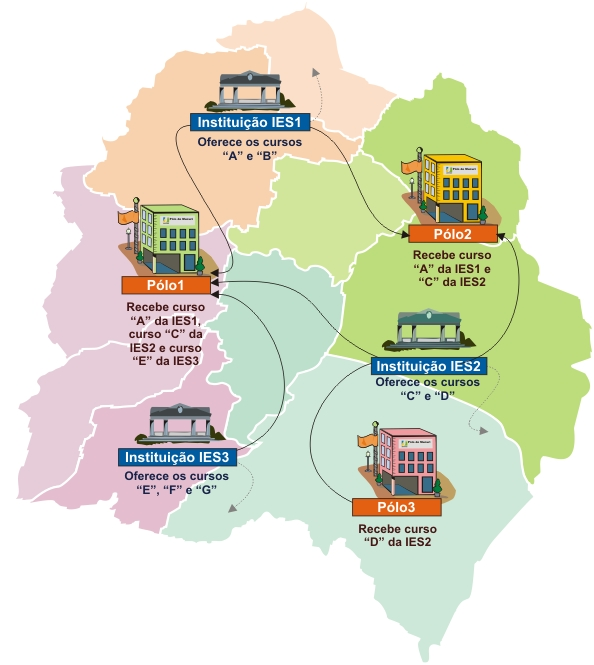
\includegraphics[width=0.35\textwidth]{imagem/cap1/fig1.jpg}}
  \caption{Cenário ilustrando as relações entre os Pólos e as Instituições de Ensino}
  \label{fig:UAB}
 \end{center}
\end{figure}

A Figura~\ref{fig:UAB}, obtida do site da UAB\footnote{\url{http://www.uab.capes.gov.br/}}, 
ilustra bem o funcionamento desta colaboração. Neste cenário, existem três instituições
de ensino e três pólos. As instituições de ensino oferecem alguns cursos para os seus 
pólos. Por exemplo, a instituição de ensino 1 (IES1) oferece o curso A ao Pólo 1 e 
o curso B ao pólo 2. Como ilustra a figura, diferentes instituições de ensino podem
compartilhar a infra-estrutura dos pólos para oferecer cursos complementares aos pólos.

Como um curso presencial, os cursos à distância tem uma grade curricular formado 
por um conjunto de disciplinas. Para o aluno se formar, este precisa passar as disciplinas
exigidas pelo curso. Numa disciplina de um curso à distância existem três tipos de educadores:
\begin{itemize}
 \item \textbf{Professores} -- Os professores são educadores que já tem experiência no ensino do tópico 
 abordado pela disciplina, tendo a ensinado em cursos presenciais ou à distância. Ele é o responsável 
 pela disciplina. Além de ter as funções usuais de um professor em uma disciplina presencial, como 
 elaborar provas, 
 o professor em uma disciplina à distância deve planejar a disciplina, acompanhar os tutores, e montar a sala de aula 
 no Ambiente Virtual de Aprendizado. O professor deve, por exemplo, criar
atividades como fóruns, pesquisas de opinião ou dever de casa.
 Em alguns cursos também é exigido que o professor visite os pólos para ter um contato mais pessoal 
 com os seus alunos e tutores, assim melhorando a interação entre esses. 
 
 \item \textbf{Tutores à Distância} -- Os tutores à distância, normalmente situados nas instituições de ensino, 
 auxiliam os professores no ensino da disciplina. Eles são responsáveis por tirar dúvidas dos alunos e ajudá-los 
 nos exercícios. Como os tutores tem um contato maior com os alunos, percebendo quais são as maiores 
 dificuldades dos alunos da disciplina, é função dos tutores de comunicar aos professores as suas observações para
 que o professor possa melhor planejar os próximos passos da disciplina. 
 
 
 \item \textbf{Tutores Presenciais} -- Finalmente, os tutores presenciais são educadores que estão situados nos pólos
 propocionando a relação presencial necessária para um bom aprendizado. 
Além de controlar a frequência dos alunos, os tutores  ajudam os alunos que tem
dificuldades em acessar a sala do curso no 
 \ava, aplicam as provas elaboradas pelos professores nos pólos e 
 ajudam os alunos a usarem os recursos disponíveis nos $\ava$s. \red{O que mais?}
\end{itemize}

\red{Incluir uma tabela resumindo as responsabilidades dos tutores, professores e alunos}

\section{Diferenças ao Ensino Presencial}  Existem muitas diferenças entre o ensino presencial e 
o ensino à distância. Enquanto o contato no ensino presencial entre os educadores e os seus alunos acontece de maneira síncrona, 
quer dizer, em horários bem definidos, no ensino à distância, o contato entre os educadores e os seus alunos é de maneira
assíncrona, quer dizer, pode ocorrer em qualquer momento. Essa diferença faz com que muitas vezes as estratégias de ensino usadas no ensino 
presencial, como o uso de quadro e de slides, não sejam as mais adequadas no ensino à distância. O uso de outras ferramentas, 
como fóruns e bate-papos, se torna mais importante. Outra diferença é que o \ead\ exige uma coordenação maior entre os professores, tutores
à distância e tutores presenciais. Como o professor não tem contato físico com os alunos, ele precisa da avaliação dos tutores, 
que tem um contato diário com os alunos, para modelar a sua disciplina e escolher que tipo de atividade que deve ser usada.

De fato, \avas\ são desenvolvidos com o intuito de incentivar 
a \emph{interatividade} entre alunos, tutores e professores. Esta interatividade é formentada por ferramentas 
disponíveis nos \avas\ como fóruns, salas de bate-papo, formação de grupos, realização de atividades, entre outras. 
Enquanto na aulas presenciais muitos alunos hesitam em participar devido a diversos fatores como timidez, insegurança ou 
mesmo limitações de linguagem, muitos alunos tendem a ser mais abertos a discussões em 
fóruns virtuais como evidenciado nas redes sociais como Facebook e Twitter. 

Contudo assim como nas redes sociais, a discussão num ambiente virtual pode perder o foco e não atingir 
o seu objetivo final. Portanto tanto para professores como para tutores, é importante dominar os 
tipos de ferramentas disponíveis em um \ava\ para que professores e tutores possam transmitir 
de maneira efetiva o conhecimento da disciplina aos seus alunos.


\section{Ambientes Virtuais de Aprendizado: Moodle}
\label{subsec:cap1:Moodle}

Os Ambientes Virtuais de Aprendizado (\avas) são plataformas computacionais que rodam ininterruptamente em servidores 
conectados à Internet. O objetivo de uma \ava\ é de fornecer os recursos necessários para professores, tutores 
e alunos poderem collaborar a fim de permitir a Educação de Qualidade à Distância. Um \ava\ permite ao 
professor organizar sua disciplina na forma
de uma página da Internet. Esta página pode ser acessada por seus alunos e seus tutores que podem não somente ver o 
material postado pelo professor, mas também pode participar de atividades e interagir entre si através, de 
por exemplo, salas de bate-papo. Um \ava\ favorece portanto a criação de uma \emph{comunidade virtual} cujo objetivo 
é o aprendizado e disseminação do conhecimento.\footnote{No Apêndice~\ref{sec:apendice}, 
descrevemos como alunos dos cursos à distância da \ufpb\ pode acessar o site do Moodle do instituto.}

Um requisito básico para o uso de um \ava\ é o conhecimento básico de navegação Web. É esperado que um usuário 
saiba acessar uma página na Internet. 

Por que usar um AVA, por que usar o Moodle?

% \section{Ambiente Virtuais de Aprendizagem}
% 
% Desde o início dos anos 90 professores ouvem comentários sobre a revolução que vem sendo provocada pela Internet no ensino e na aprendizagem, mas essa revolução ainda não se materializou. Em lugar disso, um novo conjunto de ferramentas, chamado LMS (Learning Management System em inglês, Sistema de Gestão de Aprendizagem em português), ou AVA como é mais conhecido (Ambiente Virtual de Aprendizagem), pode ser usado para melhorar seus cursos, tirando proveito das vantagens da Internet sem dispensar a necessidade do professor. Nos últimos dez anos, os AVAs experimentaram um crescimento e amadurecimento rápidos e são, hoje, considerados essenciais em muitas universidades e faculdades.
% 
% 
% 
% \section{Ambientes Virtuais de Aprendizagem}
% 
% AVAs são aplicações Intra/Internet que “rodam” em um servidor web\footnote{Servidor web é um computador que está ligado 7 dias na semana, 24 horas por dia, à Internet, onde estão gravados os arquivos do Ava e onde está um banco de dados que guarda as informações das disciplinas e usuários, podendo ser acessadas mediante autenticação, pelos interessados em qualquer lugar onde haja conexão com a rede mundial de computadores.}  e são acessadas por um navegador (Internet Explorer, Monzila Firefox, Google Chrome, Ópera, Safari, etc.). O servidor está, no caso geral, localizado em um departamento ou centro de processamento de uma Universidade, mas pode estar localizado em qualquer lugar do mundo. O professor e os alunos podem acessar o sistema de qualquer lugar onde haja um computador, conexão com a Internet e um navegador Web. Em termos simples, um AVA fornece ao professor ferramentas para que ele crie um curso baseado em uma ambiente Web (site), com controle de acesso de forma tal que somente os alunos do 
curso 
% possam acessar o mesmo. Além deste controle, os AVAs oferecem uma variedade de ferramentas que podem aumentar a eficácia de um curso. Pode-se, facilmente, compartilhar materiais de estudo, manter discussões síncronas e assíncronas\footnote{Síncrona: que acontece em tempo real, ao mesmo tempo para todos os participantes. Assíncrona: que não está vinculada ao tempo, ou seja, a discussão pode ocorrer em períodos de tempo distintos, quando uma participação que ocorre agora é respondida depois e assim por diante.}, aplicar testes de avaliação e pesquisas de opinião, coletar e revisar tarefas, além de registrar notas. 
% 
% \index{síncrono}
% \index{assíncrono}
% 
% \section{Recursos AVA}
% \index{Recursos}
% Os ambientes AVAs provêem os mais variados recursos educacionais, no intuito de prover maior didática e eficiência na comunicação entre alunos e professores.  Podemos analisar alguns destes recursos a seguir.
% 
% \subsection{Enviando e compartilhando materiais de estudo}
% \index{Materiais de estudo}
% A maioria dos AVAs fornece ferramentas para publicar com facilidade, textos e outros materiais de estudo. Ao invés de usar um editor HTML\footnote{Hypertext Markup Language: Linguagem de Marcação para Hipertextos, usada para dar formatação às páginas web e criar vínculos (links) entre elas.} , e então, enviar o texto para um servidor Web, usa-se um formulário para publicar conteúdos (enviar arquivos). Muitos professores costumam publicar em um site da Internet todo o material que produzem e que pode ser útil para os seus alunos. Porém estes ambientes não possuem tantos recursos didáticos como o ambiente AVA.
% 
% 
% \subsection{Fóruns e Salas de bate-papo}
% 
% \index{Fóruns e chat}
% 
% Esses recursos fornecem meios de comunicação entre o professor e os alunos fora da sala de aula. Os fóruns proporcionam mais tempo para reflexão antes que a participação aconteça e permitem manter uma discussão por um período longo de tempo. As salas de bate-papo, por outro lado, fornecem uma forma de comunicação rápida e instantânea com professores, tutores e alunos. Podem ser usados para uma discussão aberta, com tema livre, ou até mesmo para uma aula virtual. Sabe-se de um professor que, impedido de falar por motivos médicos, conduz seu curso usando salas de bate-papo para se comunicar com os alunos. Outro uso comum é aquele feito por grupos de alunos que devem produzir um trabalho e usam o bate-papo online para se organizar e discutir detalhes do trabalho.
% 
% \subsection{Testes e pesquisas de opinião}
% 
% \index{Testes e pesquisas}
% 
% Testes online e pesquisas de opinião podem ser corrigidos e processados instantaneamente. São grandes ferramentas para 
% permitir que os alunos tenham uma informação rápida e eficaz auto-avaliação sobre seu desempenho no curso. É comum hoje em dia que editoras e autores de livros texto coloquem questionários sobre os capítulos de seus livros em sítios na Internet. Podermos citar um exemplo de um professor que conduzindo um curso sobre propaganda na Universidade de São Francisco (EUA), produz um banco de questões e adota mini-testes para verificar o progresso dos alunos em seus estudos. A prova final é um teste com questões retiradas de todo o banco, de maneira aleatória.
% 
% \subsection{Coletando e revisando tarefas}
% 
% \index{Revisão de tarefas}
% 
% Coletar, corrigir e revisar tarefas (divulgando os resultados da correção com comentários) é um trabalho cansativo e maçante. Tarefas online é uma forma fácil de coletar e corrigir trabalhos dos alunos e atribuir e divulgar notas. Além disso, pesquisas indicam que o uso de ambientes online com participação anônima, para que os alunos atribuam notas a trabalhos feitos por seus colegas, aumenta a motivação e o desempenho.
% 
% \subsection{Registrando notas}
% 
% \index{Registro de notas}
% 
% Um quadro de notas online permite que os alunos tenham informações sempre atualizadas sobre seu desempenho em um curso. Notas online também facilitam cumprir a determinação de algumas instituições de ensino de que não tornem públicas as avaliações dos alunos. Os quadros de notas dos AVAs permitem, em geral, que os alunos consultem apenas as próprias notas. É possível, ainda, copiar o quadro de notas para o computador do professor para processamentos mais elaborados. Embora seja possível encontrar (ou desenvolver) programas que façam este trabalho, um AVA tem essas ferramentas integradas em seu ambiente. 
% 
% \section{Por que usar um AVA?}
% 
% Aulas têm sido ministradas por milhares de anos sem o uso de computadores ou da Internet. O ambiente em que o professor utiliza um quadro negro, giz e conversa ainda são ferramentas dominantes no processo educacional. Embora o formato tradicional, ou seja, de forma presencial, possa ainda ser eficaz, o uso das ferramentas acima listadas abrem novas possibilidades de aprendizagem que não eram imagináveis há anos atrás.
% 
% No momento, uma grande quantidade de pesquisa ainda é feita sobre como combinar aprendizagem presencial com os chamados cursos híbridos. Que são os cursos que combinam aulas presenciais e aula à distância. Imagine transferir a maior parte do material didático de seu curso para um ambiente virtual e aproveitar seu tempo em aula para discussões, questões e resolução de problemas. Muitos professores já descobriram que eles podem economizar tempo e melhorar a aprendizagem de seus alunos comportando-se dessa maneira. Isto permite que os alunos usem os encontros presencias para a solução de problemas e os professores possam transformar suas aulas em palestras de contextualização, abandonando a preocupação de ter que cumprir o programa de forma presencial.
% 
% As discussões online permitem que muitos alunos se expressem em formas que eles não conseguiriam em aulas regulares. Muitos deles relutam em falar em aula por motivos variados: timidez, insegurança, ou mesmo limitações de linguagem. A possibilidade de criar um ambiente de construção coletiva do conhecimento online é, muitas vezes, de grande importância para alguns alunos. Muitos professores relatam um aumento significativo na participação quando se introduz esse formato de aprendizagem. Há outro número de razões para se pensar na utilização de ambientes virtuais em seus cursos, como por exemplo:
% 
% \begin{itemize}
%  \item Demanda dos alunos: os alunos (especialmente os de curso superior) têm, hoje, um grau de inclusão digital muito maior, e utilizam muitos sistemas de comunicação como (MSN, Facebook, GTalk, Skype, por exemplo) eles se sentem à vontade em um AVA;
%  \item Horários dos alunos: aumenta cada vez mais o número de alunos que trabalha. Em alguns países, a média semanal de trabalho dos alunos de cursos superiores chega a 20 horas. Com ambientes online eles podem adequar seus horários de trabalho às atividades de um curso;
%  \item Cursos melhores: se bem usado, um AVA pode tornar suas aulas mais eficazes e melhores. Movendo parte de seu curso para a Internet é possível aproveitar os encontros presenciais para envolver os alunos em questões básicas do curso e convidá-lo a refletir sobre temas correlatos. O professor pode, também, aproveitar o tempo discorrendo sobre temas que sempre desejou abordar e foi impedido pelo fato de ter que cumprir o programa.
% \end{itemize}
% 
% Você provavelmente ouviu os argumentos até aqui apresentados durante a última década do século XX. Então, o que mudou? Hoje, os AVAs estão melhores estruturados, mais maduros, e fáceis de usar do que foram há alguns anos atrás. A tecnologia que envolve a disponibilidade deste ambiente tornou-se melhor e mais estável. Há pouco tempo, muitos sistemas eram projetados para uso pessoal, ou para uso de um grupo específico de pessoas, e eram comercializados na forma original, mostrando-se pouco flexíveis. Dois dos sistemas mais conhecidos (Blackboard e WebCT) começaram como projetos para pequenas faculdades e se tornaram líderes do mercado.
% 
% Entretanto, liderar o mercado não significa ser o melhor ou mais bem projetado. De fato, os líderes de mercado têm tido dificuldades para manter seu crescimento e argumenta-se inclusive que o esforço para manter essa liderança tem prejudicado a qualidade final do produto.
% 
% 
% 
% \section{Por que o Moodle é diferente?}
% 
% Muitos administradores de ambientes de aprendizagem têm declarado sua adesão ao Moodle principalmente em virtude de ser ele um sistema aberto baseado em uma forte filosofia educacional com uma comunidade de usuários que cresce dia a dia e contribui para o desenvolvimento e apoio a novos usuários. A seguir podem-se analisar detalhadamente algumas vantagens do AVA Moodle.
% 
% \section{Gratuito e de fonte aberta (código aberto)}
% 
% A expressão fonte aberta (do inglês open source) tornou-se um termo restrito a certo círculo de pessoas. Para aqueles que não estão acostumados com a linguagem técnica é difícil entender como essa idéia estranha e poderosa mudou para sempre o mundo do desenvolvimento de programas para computador. A idéia em si é bastante simples: fonte aberta significa que os usuários têm acesso ao código fonte do programa. Pode-se examinar (alterar, ampliar, modificar) o programa ou mesmo usar partes dele para aplicações de interesse pessoal.
% 
% Programas para computador de fonte aberta adotam valores acadêmicos de liberdade, avaliação pelos pares e compartilhamento do conhecimento. Qualquer pessoa pode baixar o Moodle gratuitamente, modificar ou acrescentar módulos, corrigir erros, melhorar seu desempenho ou simplesmente aprender observando como outras pessoas usam o ambiente e resolvem problemas. Alem disso, ao contrário dos sistemas proprietários, o Moodle pode ser instalado sem nenhum custo (em quantos servidores você desejar). Ninguém poderá retirá-lo de você, aumentar os custos de manutenção ou fazê-lo pagar por atualizações. Ninguém pode forçá-lo a fazer atualizações, comprar ferramentas que você não deseja ou determinar quantos usuários você pode ter.
% 
% 
% \section{Pedagogia}
% 
% O criador do Moodle, Martin Dougiamas, tem formação em educação e informática. Isto o conduziu a adotar o Construcionismo Social como a estrutura pedagógica em que está baseado o ambiente. Isto é inovador uma vez que os ambientes de gestão de aprendizagem são, em geral, construídos em torno de ferramentas computacionais. Pode-se afirmar que os AVAs comerciais são voltados para ferramentas enquanto o Moodle é voltado para aprendizagem. O Construcionismo Social baseia-se na idéia de que pessoas aprendem melhor quando engajadas em um processo social de construção do conhecimento, pelo ato de construir alguma coisa para outros. Este é um conceito um tanto sintético que pode ser mais bem detalhado. O termo processo social sugere que a aprendizagem é alguma coisa que se faz em grupos. Deste ponto de vista, aprendizagem é um processo de negociação de significados em uma cultura de símbolos e artefatos compartilhados. O processo de negociação de significados e utilização de recursos compartilhados é o processo de 
% construção do conhecimento. Nós não somos um quadro branco quando entramos no processo de aprendizagem. Nós precisamos testar nossos novos conhecimentos comparando-os com velhas crenças e incorporando-os em nossas estruturas de conhecimento já existentes. Parte do processo de teste e negociação envolve a criação de artefatos e símbolos para que outros interajam com eles.
% 
% E como isto tem relação com o ambiente Moodle? A primeira indicação está na interface. Enquanto AVAs centrados em ferramentas fornecem uma lista de ferramentas como sendo a interface, o ambiente Moodle coloca as ferramentas em uma interface que faz da aprendizagem a tarefa central. Pode-se estruturar um curso no ambiente Moodle nos formatos semanal, tópicos ou social. Além disso, enquanto outros AVAs se estruturam em um modelo de conteúdo que encoraja os professores a carregar uma infinidade de conteúdos estáticos, o ambiente Moodle enfoca o trabalho em ferramentas para discussão e compartilhamento de experiências. Assim, a ênfase está não em distribuir informação, mas em compartilhar idéias e engajar os alunos na construção do conhecimento.
% 
% A filosofia de projeto do Moodle torna-o um pacote amigável para professores e representa a primeira geração de ferramentas educacionais realmente úteis.
% 
% O Moodle tem uma comunidade de usuários grande e com participação na manutenção da distribuição, sugerindo sempre modificações, novas habilidades e reportando eventuais defeitos. Pode-se acessar a comunidade em  \url{http://moodle.org/}(em inglês) e no ambiente de discussão do Moodle Brasileiro em \url{http://moodle.org/?lang=pt_br em português}.
% 
% A comunidade Moodle tem sido indispensável para o sucesso do sistema. Com tantos usuários em todo o mundo sempre há alguém que pode responder a perguntas e dar conselhos. Ao mesmo tempo, os desenvolvedores e usuários do Moodle trabalham juntos para garantir qualidade, adicionar novos módulos e ferramentas e sugerir novas idéias de desenvolvimento do ambiente. Martin Dougiamas e sua equipe são responsáveis pela decisão de aceitar ou não as sugestões dos colaboradores. Em virtude do fato do ambiente ser de fonte aberta muitas pessoas desenvolvem novos módulos e os submetem à apreciação dos desenvolvedores e da comunidade. Isto funciona como um grande departamento de desenvolvimento e controle de qualidade.
% 
% Essas três vantagens - fonte aberta, Construcionismo Social e comunidade de desenvolvimento - fazem do Moodle um espaço de aprendizagem único no mundo.
% 
%                                                      \begin{flushright}Adaptação do texto do prof. Athail Rangel Pulino Filho
%                                                       
%                                                                                  Universidade de Brasília, DF\end{flushright} 
%                                                                                  

